\documentclass[a4paper,12pt]{article}
\usepackage[left=2cm,right=2cm,top=2cm,bottom=2cm]{geometry} % Do ustawień marginesów
\usepackage{multicol} % Dla podziału na kolumny
\usepackage{ragged2e} % Dla justowania tekstu
\usepackage{graphicx} % Required for inserting images
\usepackage{float}
\usepackage{caption}
\usepackage{amsmath} % Math formulas
\usepackage{amssymb} % Symbols
\usepackage[svgnames]{xcolor}
\usepackage[colorlinks=true, urlcolor=blue, linkcolor=black, citecolor=orange]{hyperref} % Hyperlinks
\usepackage{polski} % Polish language
\usepackage[utf8]{inputenc} % Text encoding
\usepackage{enumitem} % Pakiet do elastycznego sterowania listami
\usepackage{indentfirst}
\usepackage{array}

\begin{document}

% Górna część strony
\noindent
\begin{minipage}{0.5\textwidth}
    \raggedright
    \textbf{Piotr Durniat} \\
    I rok, Fizyka \\
    Wtorek, 8:00-10:15 \\
    \vspace{0.5cm}
    \vspace{0.5cm}
\end{minipage}%
\begin{minipage}{0.5\textwidth}
    \raggedleft
    Data wykonania pomiarów: \\
    08.04.2025 \\
    \vspace{0.5cm} % Dodatkowa linia przerwy
    Prowadząca: \\
    dr Iwona Mróz
\end{minipage}

% Tytuł ćwiczenia
\vspace{2cm} % Odstęp
\begin{center}
    \LARGE \textbf{Ćwiczenie nr 19} \\[0.5cm]
    \Large \textbf{Pomiary stałej grawitacji G (ważenie Ziemi)}
\end{center}

% Reszta treści
\vspace{1cm} % Kolejny odstęp
\noindent

\tableofcontents
\newpage

% ---------- WSTĘP TEORETYCZNY ----------
\section{Wstęp teoretyczny}

\subsection*{Siła grawitacji}

Siłę grawitacji $F$ dla dwóch ciał o masach $m_1$ i $m_2$ oddalonych o $r$ można wyrazić wzorem:

\begin{equation}
    F = G \frac{m_1 m_2}{r^2}
\end{equation}

gdzie:
\begin{itemize}
    \item $G$ - stała grawitacji
\end{itemize}

\subsection*{Metoda wagi skręceń Cavendisha}

Metoda wagi skręceń Cavendisha jest jedną z metod wyznaczania stałej grawitacji $G$. Waga skręceń składa się z dwóch ciężarków o masie $m$ zawieszonych na obu końcach pręta, który jest zawieszony na cienkiej sprężystej nici będącej osią obrotu. W pobliżu tych kulek umieszcza się dwa duże ciężkie kulki o masie $M$. Wówczas siła grawitacji działająca na kulki $m$ wywołuje skręcenie nici aż do momentu, w którym siła grawitacji zrównoważy siłę sprężystości nici.


% ---------- OPIS DOŚWIADCZENIA ----------
\section{Opis doświadczenia}

% ---------- OPRACOWANIE WYNIKÓW POMIARÓW ----------
\section{Opracowanie wyników pomiarów}

% ---------- TABELE ----------
\subsection{Tabele pomiarowe}

% ---------- OBLICZENIA ----------
\subsection{Wyznaczanie położeń środkowych}

\begin{align*}
    b_{01} & = \frac{\frac{b_1+b_3}{2}+b_2}{2} = \frac{b_1}{4} + \frac{b_2}{2} + \frac{b_3}{4} \rightarrow \text{pierwsze ustawienie}; \\
    b_{02} & = \frac{\frac{b_1+b_3}{2}+b_2}{2} = \frac{b_1}{4} + \frac{b_2}{2} + \frac{b_3}{4} \rightarrow \text{drugie ustawienie}.
\end{align*}

% ---------- NIEPEWNOŚCI ----------
\section{Ocena niepewności pomiaru}

\subsection{Niepewność $\Delta b$}

$$
\Delta(\Delta b) = ... 
$$

\subsection{Niepewność $T$}

$$
\Delta T = 30 s
$$

\subsection{Niepewność $G$}

Wzór (18) z instrukcji ONP:

\begin{equation}
\label{eq:delta_y}
\Delta y = \sum_{k=1}^{K} \left| \frac{\partial f}{\partial x_k} \Delta x_k \right|
\end{equation}

Wzór na stałą grawitacji:

\begin{equation}
\label{eq:g}
G = \frac{\pi^2 r^2 d \Delta b}{MT^2L}
\end{equation}

Pochodne cząstkowe:

\begin{equation}
\frac{\partial G}{\partial \Delta b} = \frac{\pi^2 r^2 d}{MT^2L} = \frac{G}{\Delta b}
\end{equation}

\begin{equation}
\frac{\partial G}{\partial \Delta T} = \frac{-2\pi^2 r^2 d}{MT^3L} = \frac{-2G}{T}
\end{equation}

Finalnie:
\begin{equation}
\Delta G = | \frac{-2G}{T} \Delta_T | + | \frac{G}{\Delta b} \Delta_{\Delta b} |
\end{equation}

















% ---------- WNIOSKI ----------
\section{Wnioski}

\newpage

% ---------- WYKRESY ----------
\section{Wykresy}

\begin{figure}[H]
    \centering
    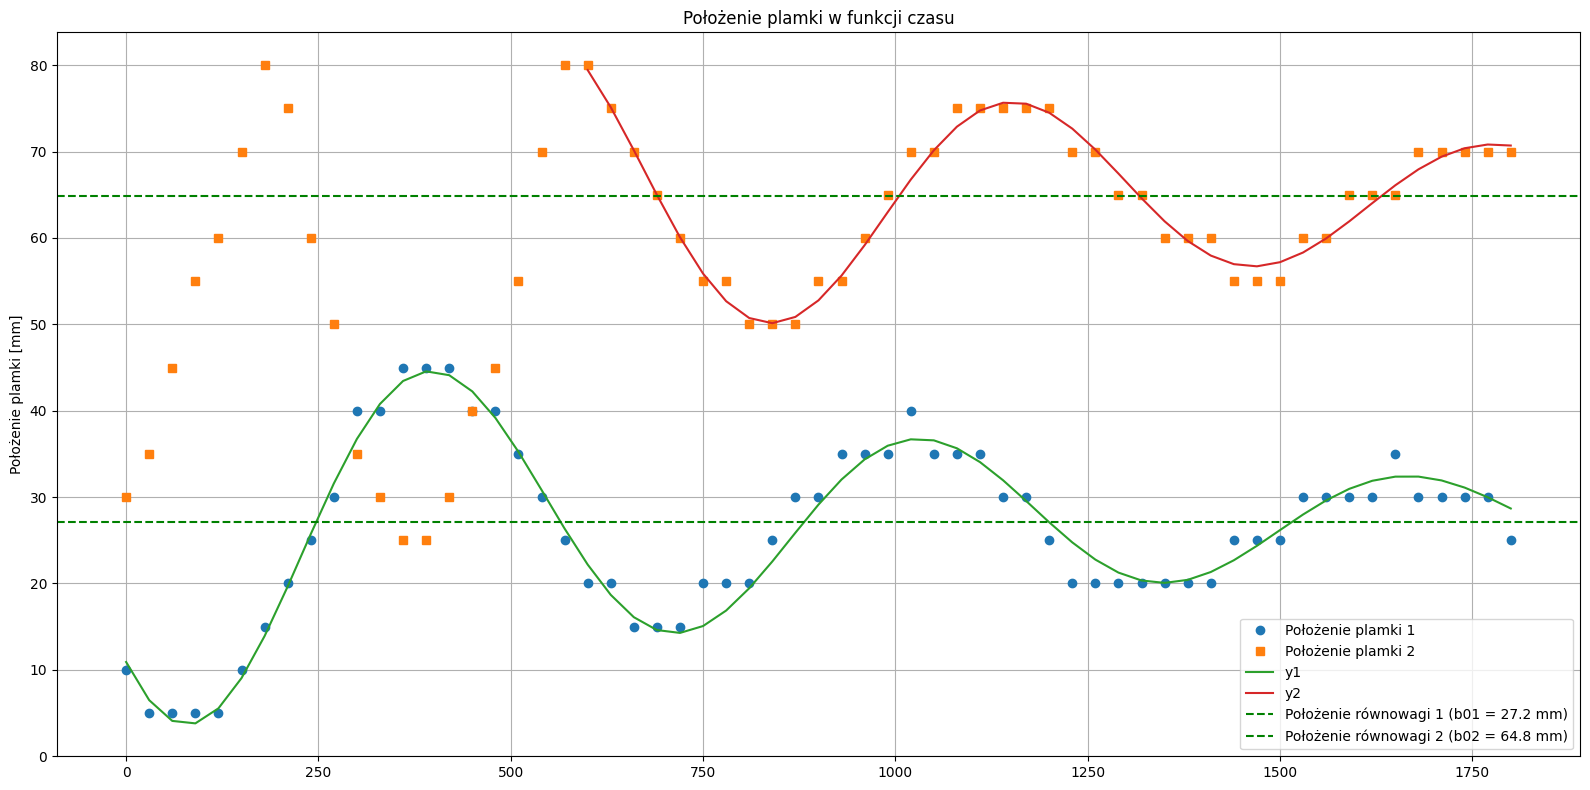
\includegraphics[width=0.9\textheight,angle=90]{wykres.png}
    \caption{Wykres zależności wychylenia od czasu}
    \label{fig:wykres}
\end{figure}


\bibliographystyle{plain}
\bibliography{bibliography}

\end{document}
